% Options for packages loaded elsewhere
\PassOptionsToPackage{unicode}{hyperref}
\PassOptionsToPackage{hyphens}{url}
%
\documentclass[
]{article}
\usepackage{amsmath,amssymb}
\usepackage{lmodern}
\usepackage{iftex}
\ifPDFTeX
  \usepackage[T1]{fontenc}
  \usepackage[utf8]{inputenc}
  \usepackage{textcomp} % provide euro and other symbols
\else % if luatex or xetex
  \usepackage{unicode-math}
  \defaultfontfeatures{Scale=MatchLowercase}
  \defaultfontfeatures[\rmfamily]{Ligatures=TeX,Scale=1}
\fi
% Use upquote if available, for straight quotes in verbatim environments
\IfFileExists{upquote.sty}{\usepackage{upquote}}{}
\IfFileExists{microtype.sty}{% use microtype if available
  \usepackage[]{microtype}
  \UseMicrotypeSet[protrusion]{basicmath} % disable protrusion for tt fonts
}{}
\makeatletter
\@ifundefined{KOMAClassName}{% if non-KOMA class
  \IfFileExists{parskip.sty}{%
    \usepackage{parskip}
  }{% else
    \setlength{\parindent}{0pt}
    \setlength{\parskip}{6pt plus 2pt minus 1pt}}
}{% if KOMA class
  \KOMAoptions{parskip=half}}
\makeatother
\usepackage{xcolor}
\usepackage[margin=1in]{geometry}
\usepackage{color}
\usepackage{fancyvrb}
\newcommand{\VerbBar}{|}
\newcommand{\VERB}{\Verb[commandchars=\\\{\}]}
\DefineVerbatimEnvironment{Highlighting}{Verbatim}{commandchars=\\\{\}}
% Add ',fontsize=\small' for more characters per line
\usepackage{framed}
\definecolor{shadecolor}{RGB}{248,248,248}
\newenvironment{Shaded}{\begin{snugshade}}{\end{snugshade}}
\newcommand{\AlertTok}[1]{\textcolor[rgb]{0.94,0.16,0.16}{#1}}
\newcommand{\AnnotationTok}[1]{\textcolor[rgb]{0.56,0.35,0.01}{\textbf{\textit{#1}}}}
\newcommand{\AttributeTok}[1]{\textcolor[rgb]{0.77,0.63,0.00}{#1}}
\newcommand{\BaseNTok}[1]{\textcolor[rgb]{0.00,0.00,0.81}{#1}}
\newcommand{\BuiltInTok}[1]{#1}
\newcommand{\CharTok}[1]{\textcolor[rgb]{0.31,0.60,0.02}{#1}}
\newcommand{\CommentTok}[1]{\textcolor[rgb]{0.56,0.35,0.01}{\textit{#1}}}
\newcommand{\CommentVarTok}[1]{\textcolor[rgb]{0.56,0.35,0.01}{\textbf{\textit{#1}}}}
\newcommand{\ConstantTok}[1]{\textcolor[rgb]{0.00,0.00,0.00}{#1}}
\newcommand{\ControlFlowTok}[1]{\textcolor[rgb]{0.13,0.29,0.53}{\textbf{#1}}}
\newcommand{\DataTypeTok}[1]{\textcolor[rgb]{0.13,0.29,0.53}{#1}}
\newcommand{\DecValTok}[1]{\textcolor[rgb]{0.00,0.00,0.81}{#1}}
\newcommand{\DocumentationTok}[1]{\textcolor[rgb]{0.56,0.35,0.01}{\textbf{\textit{#1}}}}
\newcommand{\ErrorTok}[1]{\textcolor[rgb]{0.64,0.00,0.00}{\textbf{#1}}}
\newcommand{\ExtensionTok}[1]{#1}
\newcommand{\FloatTok}[1]{\textcolor[rgb]{0.00,0.00,0.81}{#1}}
\newcommand{\FunctionTok}[1]{\textcolor[rgb]{0.00,0.00,0.00}{#1}}
\newcommand{\ImportTok}[1]{#1}
\newcommand{\InformationTok}[1]{\textcolor[rgb]{0.56,0.35,0.01}{\textbf{\textit{#1}}}}
\newcommand{\KeywordTok}[1]{\textcolor[rgb]{0.13,0.29,0.53}{\textbf{#1}}}
\newcommand{\NormalTok}[1]{#1}
\newcommand{\OperatorTok}[1]{\textcolor[rgb]{0.81,0.36,0.00}{\textbf{#1}}}
\newcommand{\OtherTok}[1]{\textcolor[rgb]{0.56,0.35,0.01}{#1}}
\newcommand{\PreprocessorTok}[1]{\textcolor[rgb]{0.56,0.35,0.01}{\textit{#1}}}
\newcommand{\RegionMarkerTok}[1]{#1}
\newcommand{\SpecialCharTok}[1]{\textcolor[rgb]{0.00,0.00,0.00}{#1}}
\newcommand{\SpecialStringTok}[1]{\textcolor[rgb]{0.31,0.60,0.02}{#1}}
\newcommand{\StringTok}[1]{\textcolor[rgb]{0.31,0.60,0.02}{#1}}
\newcommand{\VariableTok}[1]{\textcolor[rgb]{0.00,0.00,0.00}{#1}}
\newcommand{\VerbatimStringTok}[1]{\textcolor[rgb]{0.31,0.60,0.02}{#1}}
\newcommand{\WarningTok}[1]{\textcolor[rgb]{0.56,0.35,0.01}{\textbf{\textit{#1}}}}
\usepackage{longtable,booktabs,array}
\usepackage{calc} % for calculating minipage widths
% Correct order of tables after \paragraph or \subparagraph
\usepackage{etoolbox}
\makeatletter
\patchcmd\longtable{\par}{\if@noskipsec\mbox{}\fi\par}{}{}
\makeatother
% Allow footnotes in longtable head/foot
\IfFileExists{footnotehyper.sty}{\usepackage{footnotehyper}}{\usepackage{footnote}}
\makesavenoteenv{longtable}
\usepackage{graphicx}
\makeatletter
\def\maxwidth{\ifdim\Gin@nat@width>\linewidth\linewidth\else\Gin@nat@width\fi}
\def\maxheight{\ifdim\Gin@nat@height>\textheight\textheight\else\Gin@nat@height\fi}
\makeatother
% Scale images if necessary, so that they will not overflow the page
% margins by default, and it is still possible to overwrite the defaults
% using explicit options in \includegraphics[width, height, ...]{}
\setkeys{Gin}{width=\maxwidth,height=\maxheight,keepaspectratio}
% Set default figure placement to htbp
\makeatletter
\def\fps@figure{htbp}
\makeatother
\setlength{\emergencystretch}{3em} % prevent overfull lines
\providecommand{\tightlist}{%
  \setlength{\itemsep}{0pt}\setlength{\parskip}{0pt}}
\setcounter{secnumdepth}{-\maxdimen} % remove section numbering
\ifLuaTeX
  \usepackage{selnolig}  % disable illegal ligatures
\fi
\IfFileExists{bookmark.sty}{\usepackage{bookmark}}{\usepackage{hyperref}}
\IfFileExists{xurl.sty}{\usepackage{xurl}}{} % add URL line breaks if available
\urlstyle{same} % disable monospaced font for URLs
\hypersetup{
  pdftitle={DATA 621 HW 1},
  hidelinks,
  pdfcreator={LaTeX via pandoc}}

\title{DATA 621 HW 1}
\author{}
\date{\vspace{-2.5em}Last edited September 14, 2023}

\begin{document}
\maketitle

\begin{verbatim}
## Warning: package 'corrplot' was built under R version 4.2.3
\end{verbatim}

\hypertarget{business-analytics-and-data-mining}{%
\section{\texorpdfstring{\textbf{Business Analytics and Data
Mining}}{Business Analytics and Data Mining}}\label{business-analytics-and-data-mining}}

\hypertarget{homework-1-assignment-requirements}{%
\subsection{Homework \#1 Assignment
Requirements}\label{homework-1-assignment-requirements}}

\hypertarget{overview}{%
\subsubsection{\texorpdfstring{\textbf{Overview}}{Overview}}\label{overview}}

In this homework assignment, you will explore, analyze and model a data
set containing approximately 2200 records. Each record represents a
professional baseball team from the years 1871 to 2006 inclusive. Each
record has the performance of the team for the given year, with all of
the statistics adjusted to match the performance of a 162 game season.

Your objective is to build a multiple linear regression model on the
training data to predict the number of wins for the team. You can only
use the variables given to you (or variables that you derive from the
variables provided).

Below is a short description of the variables of interest in the data
set:

\begin{longtable}[]{@{}
  >{\raggedright\arraybackslash}p{(\columnwidth - 4\tabcolsep) * \real{0.2727}}
  >{\centering\arraybackslash}p{(\columnwidth - 4\tabcolsep) * \real{0.4432}}
  >{\raggedleft\arraybackslash}p{(\columnwidth - 4\tabcolsep) * \real{0.2841}}@{}}
\toprule()
\begin{minipage}[b]{\linewidth}\raggedright
Variable Names
\end{minipage} & \begin{minipage}[b]{\linewidth}\centering
Definition
\end{minipage} & \begin{minipage}[b]{\linewidth}\raggedleft
Theoretical Effect
\end{minipage} \\
\midrule()
\endhead
INDEX & Identification Variable (do not use) & None \\
TARGET\_WINS & Number of wins & \$12 \\
TEAM\_BATTING\_H & Base Hits by batters (1B,2B,3B,HR) & Positive Impact
on Wins \\
TEAM\_BATTING\_2B & Doubles by batters (2B) & Positive Impact on Wins \\
TEAM\_BATTING\_3B & Triples by batters (3B) & Positive Impact on Wins \\
TEAM\_BATTING\_HR & Homeruns by batters (4B) & Positive Impact on
Wins \\
TEAM\_BATTING\_BB & Walks by batters & Positive Impact on Wins \\
TEAM\_BATTING\_HBP & Batters hit by pitch (get a free base) & Positive
Impact on Wins \\
TEAM\_BATTING\_SO & Strikeouts by batters & Negative Impact on Wins \\
TEAM\_BASERUN\_SB & Stolen bases & Positive Impact on Wins \\
TEAM\_BASERUN\_CS & Caught stealing & Negative Impact on Wins \\
TEAM\_FIELDING\_E & Errors & Negative Impact on Wins \\
TEAM\_FIELDING\_DP & Double Plays & Positive Impact on Wins \\
TEAM\_PITCHING\_BB & Walks allowed & Negative Impact on Wins \\
TEAM\_PITCHING\_H & Hits allowed & Negative Impact on Wins \\
TEAM\_PITCHING\_HR & Homeruns allowed & Negative Impact on Wins \\
TEAM\_PITCHING\_SO & Strikeouts by pitchers & Positive Impact on Wins \\
\bottomrule()
\end{longtable}

\hypertarget{deliverable}{%
\subsubsection{\texorpdfstring{\textbf{Deliverable:}}{Deliverable:}}\label{deliverable}}

\begin{itemize}
\tightlist
\item
  A write-up submitted in PDF format. Your write-up should have four
  sections. Each one is described below. You may assume you are
  addressing me as a fellow data scientist, so do not need to shy away
  from technical details.
\item
  Assigned predictions (the number of wins for the team) for the
  evaluation data set.
\item
  Include your R statistical programming code in an Appendix.
\end{itemize}

\hypertarget{write-up}{%
\subsubsection{\texorpdfstring{\textbf{Write
Up:}}{Write Up:}}\label{write-up}}

\begin{enumerate}
\def\labelenumi{\arabic{enumi}.}
\tightlist
\item
  \textbf{DATA EXPLORATION (25 Points)} Describe the size and the
  variables in the moneyball training data set. Consider that too much
  detail will cause a manager to lose interest while too little detail
  will make the manager consider that you aren't doing your job. Some
  suggestions are given below. Please do NOT treat this as a check list
  of things to do to complete the assignment. You should have your own
  thoughts on what to tell the boss. These are just ideas.
\end{enumerate}

\begin{enumerate}
\def\labelenumi{\alph{enumi}.}
\tightlist
\item
  Mean / Standard Deviation / Median
\item
  Bar Chart or Box Plot of the data
\item
  Is the data correlated to the target variable (or to other variables?)
\item
  Are any of the variables missing and need to be imputed ``fixed''?
\end{enumerate}

\begin{enumerate}
\def\labelenumi{\arabic{enumi}.}
\setcounter{enumi}{1}
\tightlist
\item
  \textbf{DATA PREPARATION (25 Points)} Describe how you have
  transformed the data by changing the original variables or creating
  new variables. If you did transform the data or create new variables,
  discuss why you did this. Here are some possible transformations.
\end{enumerate}

\begin{enumerate}
\def\labelenumi{\alph{enumi}.}
\tightlist
\item
  Fix missing values (maybe with a Mean or Median value)
\item
  Create flags to suggest if a variable was missing
\item
  Transform data by putting it into buckets
\item
  Mathematical transforms such as log or square root (or use Box-Cox)
\item
  Combine variables (such as ratios or adding or multiplying) to create
  new variables
\end{enumerate}

\begin{enumerate}
\def\labelenumi{\arabic{enumi}.}
\setcounter{enumi}{2}
\item
  \textbf{BUILD MODELS (25 Points)} Using the training data set, build
  at least three different multiple linear regression models, using
  different variables (or the same variables with different
  transformations). Since we have not yet covered automated variable
  selection methods, you should select the variables manually (unless
  you previously learned Forward or Stepwise selection, etc.). Since you
  manually selected a variable for inclusion into the model or exclusion
  into the model, indicate why this was done. Discuss the coefficients
  in the models, do they make sense? For example, if a team hits a lot
  of Home Runs, it would be reasonably expected that such a team would
  win more games. However, if the coefficient is negative (suggesting
  that the team would lose more games), then that needs to be discussed.
  Are you keeping the model even though it is counter intuitive? Why?
  The boss needs to know.
\item
  \textbf{SELECT MODELS (25 Points)} Decide on the criteria for
  selecting the best multiple linear regression model. Will you select a
  model with slightly worse performance if it makes more sense or is
  more parsimonious? Discuss why you selected your model. For the
  multiple linear regression model, will you use a metric such as
  Adjusted R2 , RMSE, etc.? Be sure to explain how you can make
  inferences from the model, discuss multi-collinearity issues (if any),
  and discuss other relevant model output. Using the training data set,
  evaluate the multiple linear regression model based on (a) mean
  squared error, (b) R2, (c) F-statistic, and (d) residual plots. Make
  predictions using the evaluation data set.
\end{enumerate}

\newpage

\hypertarget{evaluation}{%
\subsection{\texorpdfstring{\textbf{Evaluation}}{Evaluation}}\label{evaluation}}

\hypertarget{load-the-data}{%
\subsubsection{\texorpdfstring{\textbf{Load the
data}}{Load the data}}\label{load-the-data}}

\begin{Shaded}
\begin{Highlighting}[]
\NormalTok{git\_url}\OtherTok{\textless{}{-}}
  \StringTok{"https://raw.githubusercontent.com/melbow2424/Data621\_HW1/main/"}

\NormalTok{df\_train }\OtherTok{\textless{}{-}} 
  \FunctionTok{read.csv}\NormalTok{(}\FunctionTok{paste0}\NormalTok{(git\_url,}\StringTok{"moneyball{-}training{-}data.csv"}\NormalTok{))}

\NormalTok{df\_evaluation }\OtherTok{\textless{}{-}} 
  \FunctionTok{read.csv}\NormalTok{(}\FunctionTok{paste0}\NormalTok{(git\_url,}\StringTok{"moneyball{-}evaluation{-}data.csv"}\NormalTok{))}
\end{Highlighting}
\end{Shaded}

\hypertarget{data-exploration}{%
\subsubsection{1. Data Exploration**}\label{data-exploration}}

\begin{Shaded}
\begin{Highlighting}[]
\FunctionTok{print}\NormalTok{(}\FunctionTok{skim}\NormalTok{(df\_train))}
\end{Highlighting}
\end{Shaded}

\begin{verbatim}
## -- Data Summary ------------------------
##                            Values  
## Name                       df_train
## Number of rows             2276    
## Number of columns          17      
## _______________________            
## Column type frequency:             
##   numeric                  17      
## ________________________           
## Group variables            None    
## 
## -- Variable type: numeric ------------------------------------------------------
##    skim_variable    n_missing complete_rate   mean     sd   p0    p25   p50
##  1 INDEX                    0        1      1268.   736.     1  631.  1270.
##  2 TARGET_WINS              0        1        80.8   15.8    0   71     82 
##  3 TEAM_BATTING_H           0        1      1469.   145.   891 1383   1454 
##  4 TEAM_BATTING_2B          0        1       241.    46.8   69  208    238 
##  5 TEAM_BATTING_3B          0        1        55.2   27.9    0   34     47 
##  6 TEAM_BATTING_HR          0        1        99.6   60.5    0   42    102 
##  7 TEAM_BATTING_BB          0        1       502.   123.     0  451    512 
##  8 TEAM_BATTING_SO        102        0.955   736.   249.     0  548    750 
##  9 TEAM_BASERUN_SB        131        0.942   125.    87.8    0   66    101 
## 10 TEAM_BASERUN_CS        772        0.661    52.8   23.0    0   38     49 
## 11 TEAM_BATTING_HBP      2085        0.0839   59.4   13.0   29   50.5   58 
## 12 TEAM_PITCHING_H          0        1      1779.  1407.  1137 1419   1518 
## 13 TEAM_PITCHING_HR         0        1       106.    61.3    0   50    107 
## 14 TEAM_PITCHING_BB         0        1       553.   166.     0  476    536.
## 15 TEAM_PITCHING_SO       102        0.955   818.   553.     0  615    814.
## 16 TEAM_FIELDING_E          0        1       246.   228.    65  127    159 
## 17 TEAM_FIELDING_DP       286        0.874   146.    26.2   52  131    149 
##      p75  p100 hist 
##  1 1916.  2535 ▇▇▇▇▇
##  2   92    146 ▁▁▇▅▁
##  3 1537.  2554 ▁▇▂▁▁
##  4  273    458 ▁▆▇▂▁
##  5   72    223 ▇▇▂▁▁
##  6  147    264 ▇▆▇▅▁
##  7  580    878 ▁▁▇▇▁
##  8  930   1399 ▁▆▇▇▁
##  9  156    697 ▇▃▁▁▁
## 10   62    201 ▃▇▁▁▁
## 11   67     95 ▂▇▇▅▁
## 12 1682. 30132 ▇▁▁▁▁
## 13  150    343 ▇▇▆▁▁
## 14  611   3645 ▇▁▁▁▁
## 15  968  19278 ▇▁▁▁▁
## 16  249.  1898 ▇▁▁▁▁
## 17  164    228 ▁▂▇▆▁
\end{verbatim}

Histograms a good way to visualize the distributions of the original
variables.

\begin{Shaded}
\begin{Highlighting}[]
\NormalTok{df\_train }\SpecialCharTok{\%\textgreater{}\%} 
  \FunctionTok{gather}\NormalTok{(variable, value, TARGET\_WINS}\SpecialCharTok{:}\NormalTok{ TEAM\_FIELDING\_DP)}\SpecialCharTok{\%\textgreater{}\%} \CommentTok{\#pivot longer to plot all variables}
  \FunctionTok{ggplot}\NormalTok{(.,}\FunctionTok{aes}\NormalTok{(}\AttributeTok{x=}\NormalTok{value)) }\SpecialCharTok{+} \CommentTok{\#plotting every variable}
  \FunctionTok{geom\_density}\NormalTok{(}\AttributeTok{fill =} \StringTok{"darkgreen"}\NormalTok{, }\AttributeTok{alpha =} \FloatTok{0.5}\NormalTok{) }\SpecialCharTok{+}
  \FunctionTok{facet\_wrap}\NormalTok{(}\SpecialCharTok{\textasciitilde{}}\NormalTok{ variable, }\AttributeTok{scales =} \StringTok{"free"}\NormalTok{, }\AttributeTok{ncol =} \DecValTok{4}\NormalTok{) }\SpecialCharTok{+}
  \FunctionTok{theme\_classic}\NormalTok{()}
\end{Highlighting}
\end{Shaded}

\begin{verbatim}
## Warning: Removed 3478 rows containing non-finite values (`stat_density()`).
\end{verbatim}

\includegraphics{Data_621_HW_1_files/figure-latex/unnamed-chunk-4-1.pdf}
\#\#\#\#\# Initial Observations * The response variable
\textbf{TARGET\_WINS} appears normally distributed * Several variables
such as \textbf{TEAM\_BATTING\_SO} appear to be bimodal, which may
resolve after the missing data is dealt with * Other variables like
\textbf{TEAM\_PITCHING\_H} appear to be skewed far left and may present
a challenge unless imputation of missing values corrects this

\hypertarget{get-the-means-of-columns-in-data}{%
\paragraph{\texorpdfstring{\textbf{Get the Means of columns in
Data}}{Get the Means of columns in Data}}\label{get-the-means-of-columns-in-data}}

\begin{Shaded}
\begin{Highlighting}[]
\NormalTok{train\_means}\OtherTok{\textless{}{-}}\FunctionTok{sapply}\NormalTok{(df\_train, }\ControlFlowTok{function}\NormalTok{(x) }\FunctionTok{round}\NormalTok{(}\FunctionTok{mean}\NormalTok{(x, }\AttributeTok{na.rm =} \ConstantTok{TRUE}\NormalTok{)))}
\NormalTok{train\_means}
\end{Highlighting}
\end{Shaded}

\begin{verbatim}
##            INDEX      TARGET_WINS   TEAM_BATTING_H  TEAM_BATTING_2B 
##             1268               81             1469              241 
##  TEAM_BATTING_3B  TEAM_BATTING_HR  TEAM_BATTING_BB  TEAM_BATTING_SO 
##               55              100              502              736 
##  TEAM_BASERUN_SB  TEAM_BASERUN_CS TEAM_BATTING_HBP  TEAM_PITCHING_H 
##              125               53               59             1779 
## TEAM_PITCHING_HR TEAM_PITCHING_BB TEAM_PITCHING_SO  TEAM_FIELDING_E 
##              106              553              818              246 
## TEAM_FIELDING_DP 
##              146
\end{verbatim}

\begin{Shaded}
\begin{Highlighting}[]
\NormalTok{eval\_means}\OtherTok{\textless{}{-}}\FunctionTok{sapply}\NormalTok{(df\_evaluation, }\ControlFlowTok{function}\NormalTok{(x) }\FunctionTok{round}\NormalTok{(}\FunctionTok{mean}\NormalTok{(x, }\AttributeTok{na.rm =} \ConstantTok{TRUE}\NormalTok{)))}
\NormalTok{eval\_means}
\end{Highlighting}
\end{Shaded}

\begin{verbatim}
##            INDEX   TEAM_BATTING_H  TEAM_BATTING_2B  TEAM_BATTING_3B 
##             1264             1469              241               56 
##  TEAM_BATTING_HR  TEAM_BATTING_BB  TEAM_BATTING_SO  TEAM_BASERUN_SB 
##               96              499              709              124 
##  TEAM_BASERUN_CS TEAM_BATTING_HBP  TEAM_PITCHING_H TEAM_PITCHING_HR 
##               52               62             1813              102 
## TEAM_PITCHING_BB TEAM_PITCHING_SO  TEAM_FIELDING_E TEAM_FIELDING_DP 
##              552              800              250              146
\end{verbatim}

\hypertarget{get-the-medians-of-columns-in-data}{%
\paragraph{\texorpdfstring{\textbf{Get the Medians of columns in
data}}{Get the Medians of columns in data}}\label{get-the-medians-of-columns-in-data}}

\begin{Shaded}
\begin{Highlighting}[]
\NormalTok{train\_medians}\OtherTok{\textless{}{-}}\FunctionTok{sapply}\NormalTok{(df\_train, }\ControlFlowTok{function}\NormalTok{(x) }\FunctionTok{round}\NormalTok{(}\FunctionTok{median}\NormalTok{(x, }\AttributeTok{na.rm =} \ConstantTok{TRUE}\NormalTok{)))}
\NormalTok{train\_medians}
\end{Highlighting}
\end{Shaded}

\begin{verbatim}
##            INDEX      TARGET_WINS   TEAM_BATTING_H  TEAM_BATTING_2B 
##             1270               82             1454              238 
##  TEAM_BATTING_3B  TEAM_BATTING_HR  TEAM_BATTING_BB  TEAM_BATTING_SO 
##               47              102              512              750 
##  TEAM_BASERUN_SB  TEAM_BASERUN_CS TEAM_BATTING_HBP  TEAM_PITCHING_H 
##              101               49               58             1518 
## TEAM_PITCHING_HR TEAM_PITCHING_BB TEAM_PITCHING_SO  TEAM_FIELDING_E 
##              107              536              814              159 
## TEAM_FIELDING_DP 
##              149
\end{verbatim}

\begin{Shaded}
\begin{Highlighting}[]
\NormalTok{eval\_medians}\OtherTok{\textless{}{-}}\FunctionTok{sapply}\NormalTok{(df\_evaluation, }\ControlFlowTok{function}\NormalTok{(x) }\FunctionTok{round}\NormalTok{(}\FunctionTok{median}\NormalTok{(x, }\AttributeTok{na.rm =} \ConstantTok{TRUE}\NormalTok{)))}
\NormalTok{eval\_medians}
\end{Highlighting}
\end{Shaded}

\begin{verbatim}
##            INDEX   TEAM_BATTING_H  TEAM_BATTING_2B  TEAM_BATTING_3B 
##             1249             1455              239               52 
##  TEAM_BATTING_HR  TEAM_BATTING_BB  TEAM_BATTING_SO  TEAM_BASERUN_SB 
##              101              509              686               92 
##  TEAM_BASERUN_CS TEAM_BATTING_HBP  TEAM_PITCHING_H TEAM_PITCHING_HR 
##               50               62             1515              104 
## TEAM_PITCHING_BB TEAM_PITCHING_SO  TEAM_FIELDING_E TEAM_FIELDING_DP 
##              526              745              163              148
\end{verbatim}

\hypertarget{replace-na-values-in-columns-with-their-respective-mean}{%
\paragraph{\texorpdfstring{\textbf{Replace NA values in columns with
their respective
Mean}}{Replace NA values in columns with their respective Mean}}\label{replace-na-values-in-columns-with-their-respective-mean}}

Made new copies of Train and Evaluation datasets, with imputed means.

\begin{Shaded}
\begin{Highlighting}[]
\CommentTok{\# Replace NA values in \textquotesingle{}column\_name\textquotesingle{} with \textquotesingle{}mean\textquotesingle{}}
\NormalTok{df\_train\_mn }\OtherTok{\textless{}{-}}\NormalTok{ df\_train }\SpecialCharTok{\%\textgreater{}\%}
  \FunctionTok{mutate}\NormalTok{(}\AttributeTok{TEAM\_BATTING\_SO =}
           \FunctionTok{ifelse}\NormalTok{(}\FunctionTok{is.na}\NormalTok{(TEAM\_BATTING\_SO),}
\NormalTok{                  train\_means[}\DecValTok{8}\NormalTok{],TEAM\_BATTING\_SO))}\SpecialCharTok{\%\textgreater{}\%} 
  \FunctionTok{mutate}\NormalTok{(}\AttributeTok{TEAM\_BASERUN\_SB =} 
           \FunctionTok{ifelse}\NormalTok{(}\FunctionTok{is.na}\NormalTok{(TEAM\_BASERUN\_SB),}
\NormalTok{                  train\_means[}\DecValTok{9}\NormalTok{], TEAM\_BASERUN\_SB))}\SpecialCharTok{\%\textgreater{}\%}
  \FunctionTok{mutate}\NormalTok{(}\AttributeTok{TEAM\_BASERUN\_CS =}
           \FunctionTok{ifelse}\NormalTok{(}\FunctionTok{is.na}\NormalTok{(TEAM\_BASERUN\_CS),}
\NormalTok{                  train\_means[}\DecValTok{10}\NormalTok{], TEAM\_BASERUN\_CS))}\SpecialCharTok{\%\textgreater{}\%}
  \FunctionTok{mutate}\NormalTok{(}\AttributeTok{TEAM\_BATTING\_HBP =} 
           \FunctionTok{ifelse}\NormalTok{(}\FunctionTok{is.na}\NormalTok{(TEAM\_BATTING\_HBP),}
\NormalTok{                  train\_means[}\DecValTok{11}\NormalTok{],TEAM\_BATTING\_HBP))}\SpecialCharTok{\%\textgreater{}\%}
  \FunctionTok{mutate}\NormalTok{(}\AttributeTok{TEAM\_PITCHING\_SO =}
           \FunctionTok{ifelse}\NormalTok{(}\FunctionTok{is.na}\NormalTok{(TEAM\_PITCHING\_SO),}
\NormalTok{                  train\_means[}\DecValTok{15}\NormalTok{], TEAM\_PITCHING\_SO))}\SpecialCharTok{\%\textgreater{}\%}
  \FunctionTok{mutate}\NormalTok{(}\AttributeTok{TEAM\_FIELDING\_DP =}
           \FunctionTok{ifelse}\NormalTok{(}\FunctionTok{is.na}\NormalTok{(TEAM\_FIELDING\_DP),}
\NormalTok{                  train\_means[}\DecValTok{17}\NormalTok{], TEAM\_FIELDING\_DP))}
\end{Highlighting}
\end{Shaded}

\begin{Shaded}
\begin{Highlighting}[]
\NormalTok{df\_train\_mn }\SpecialCharTok{\%\textgreater{}\%} 
  \FunctionTok{gather}\NormalTok{(variable, value, TARGET\_WINS}\SpecialCharTok{:}\NormalTok{ TEAM\_FIELDING\_DP)}\SpecialCharTok{\%\textgreater{}\%} \CommentTok{\#pivot longer to plot all variables}
  \FunctionTok{ggplot}\NormalTok{(.,}\FunctionTok{aes}\NormalTok{(}\AttributeTok{x=}\NormalTok{value)) }\SpecialCharTok{+} \CommentTok{\#plotting every variable}
  \FunctionTok{geom\_density}\NormalTok{(}\AttributeTok{fill =} \StringTok{"darkgreen"}\NormalTok{, }\AttributeTok{alpha =} \FloatTok{0.5}\NormalTok{) }\SpecialCharTok{+}
  \FunctionTok{facet\_wrap}\NormalTok{(}\SpecialCharTok{\textasciitilde{}}\NormalTok{ variable, }\AttributeTok{scales =} \StringTok{"free"}\NormalTok{, }\AttributeTok{ncol =} \DecValTok{4}\NormalTok{) }\SpecialCharTok{+}
  \FunctionTok{theme\_classic}\NormalTok{()}
\end{Highlighting}
\end{Shaded}

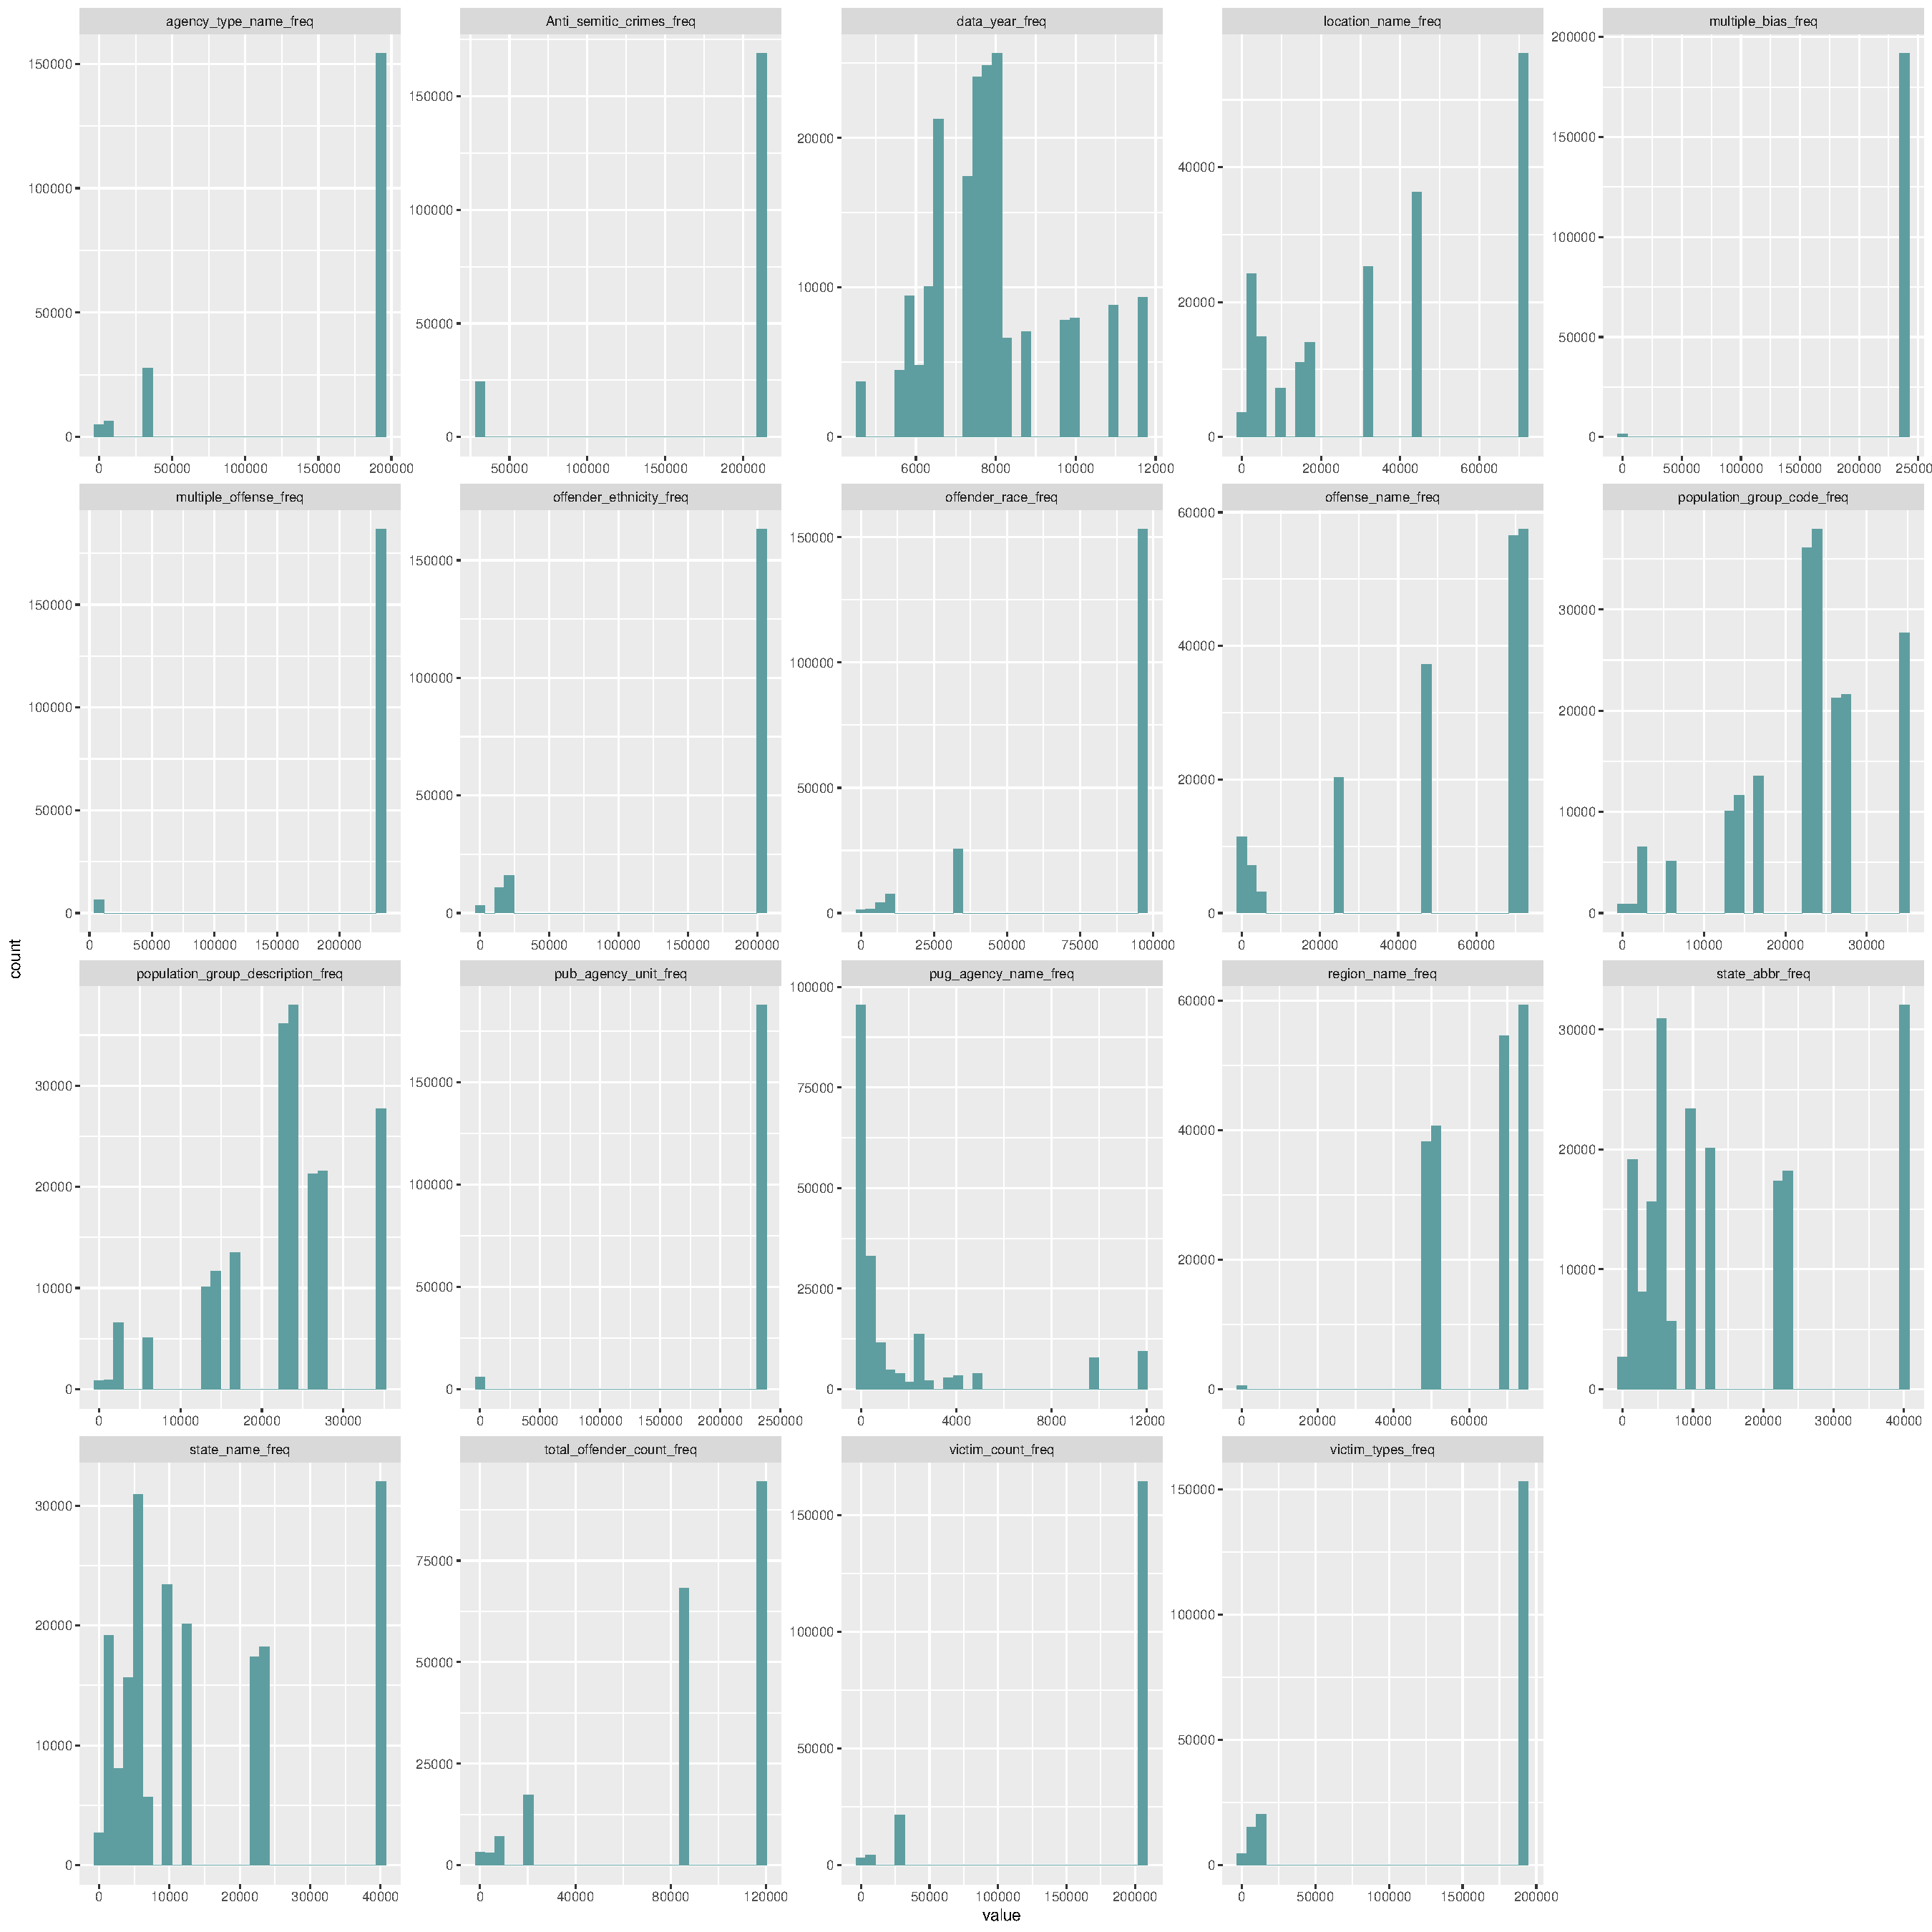
\includegraphics{Data_621_HW_1_files/figure-latex/unnamed-chunk-10-1.pdf}
\#\#\#\#\# Observations after imputation with the mean * The response
variable \textbf{TARGET\_WINS} still appears normally distributed * The
bimodality of the \textbf{TEAM\_BATTING} variables is largely unresolved
* The far left skew of the \textbf{TEAM\_PITCHING} variables is largely
unresolved

\begin{Shaded}
\begin{Highlighting}[]
\NormalTok{df\_evaluation\_mn }\OtherTok{\textless{}{-}}\NormalTok{ df\_evaluation }\SpecialCharTok{\%\textgreater{}\%}
  \FunctionTok{mutate}\NormalTok{(}\AttributeTok{TEAM\_BATTING\_SO =}
           \FunctionTok{ifelse}\NormalTok{(}\FunctionTok{is.na}\NormalTok{(TEAM\_BATTING\_SO),}
\NormalTok{                  eval\_means[}\DecValTok{8}\NormalTok{],TEAM\_BATTING\_SO))}\SpecialCharTok{\%\textgreater{}\%} 
  \FunctionTok{mutate}\NormalTok{(}\AttributeTok{TEAM\_BASERUN\_SB =} 
           \FunctionTok{ifelse}\NormalTok{(}\FunctionTok{is.na}\NormalTok{(TEAM\_BASERUN\_SB),}
\NormalTok{                  eval\_means[}\DecValTok{9}\NormalTok{], TEAM\_BASERUN\_SB))}\SpecialCharTok{\%\textgreater{}\%}
  \FunctionTok{mutate}\NormalTok{(}\AttributeTok{TEAM\_BASERUN\_CS =}
           \FunctionTok{ifelse}\NormalTok{(}\FunctionTok{is.na}\NormalTok{(TEAM\_BASERUN\_CS),}
\NormalTok{                  eval\_means[}\DecValTok{10}\NormalTok{], TEAM\_BASERUN\_CS))}\SpecialCharTok{\%\textgreater{}\%}
  \FunctionTok{mutate}\NormalTok{(}\AttributeTok{TEAM\_BATTING\_HBP =} 
           \FunctionTok{ifelse}\NormalTok{(}\FunctionTok{is.na}\NormalTok{(TEAM\_BATTING\_HBP),}
\NormalTok{                  eval\_means[}\DecValTok{11}\NormalTok{],TEAM\_BATTING\_HBP))}\SpecialCharTok{\%\textgreater{}\%}
  \FunctionTok{mutate}\NormalTok{(}\AttributeTok{TEAM\_PITCHING\_SO =}
           \FunctionTok{ifelse}\NormalTok{(}\FunctionTok{is.na}\NormalTok{(TEAM\_PITCHING\_SO),}
\NormalTok{                  eval\_means[}\DecValTok{15}\NormalTok{], TEAM\_PITCHING\_SO))}\SpecialCharTok{\%\textgreater{}\%}
  \FunctionTok{mutate}\NormalTok{(}\AttributeTok{TEAM\_FIELDING\_DP =}
           \FunctionTok{ifelse}\NormalTok{(}\FunctionTok{is.na}\NormalTok{(TEAM\_FIELDING\_DP),}
\NormalTok{                  eval\_means[}\DecValTok{17}\NormalTok{], TEAM\_FIELDING\_DP))}
\end{Highlighting}
\end{Shaded}

\hypertarget{replace-na-values-with-their-respective-medians}{%
\paragraph{\texorpdfstring{\textbf{Replace NA values with their
respective
Medians}}{Replace NA values with their respective Medians}}\label{replace-na-values-with-their-respective-medians}}

Made new copies of Train and Evaluation datasets, with imputed median.

\begin{Shaded}
\begin{Highlighting}[]
\CommentTok{\# Replace NA values in \textquotesingle{}column\_name\textquotesingle{} with \textquotesingle{}median\textquotesingle{}}
\NormalTok{df\_train\_md }\OtherTok{\textless{}{-}}\NormalTok{ df\_train }\SpecialCharTok{\%\textgreater{}\%}
  \FunctionTok{mutate}\NormalTok{(}\AttributeTok{TEAM\_BATTING\_SO =}
           \FunctionTok{ifelse}\NormalTok{(}\FunctionTok{is.na}\NormalTok{(TEAM\_BATTING\_SO),}
\NormalTok{                  train\_medians[}\DecValTok{8}\NormalTok{],TEAM\_BATTING\_SO))}\SpecialCharTok{\%\textgreater{}\%}
  \FunctionTok{mutate}\NormalTok{(}\AttributeTok{TEAM\_BASERUN\_SB =}
           \FunctionTok{ifelse}\NormalTok{(}\FunctionTok{is.na}\NormalTok{(TEAM\_BASERUN\_SB),}
\NormalTok{                  train\_medians[}\DecValTok{9}\NormalTok{], TEAM\_BASERUN\_SB))}\SpecialCharTok{\%\textgreater{}\%}
  \FunctionTok{mutate}\NormalTok{(}\AttributeTok{TEAM\_BASERUN\_CS =}
           \FunctionTok{ifelse}\NormalTok{(}\FunctionTok{is.na}\NormalTok{(TEAM\_BASERUN\_CS),}
\NormalTok{                  train\_medians[}\DecValTok{10}\NormalTok{], TEAM\_BASERUN\_CS))}\SpecialCharTok{\%\textgreater{}\%}
  \FunctionTok{mutate}\NormalTok{(}\AttributeTok{TEAM\_BATTING\_HBP =}
           \FunctionTok{ifelse}\NormalTok{(}\FunctionTok{is.na}\NormalTok{(TEAM\_BATTING\_HBP),}
\NormalTok{                  train\_medians[}\DecValTok{11}\NormalTok{],TEAM\_BATTING\_HBP))}\SpecialCharTok{\%\textgreater{}\%}
  \FunctionTok{mutate}\NormalTok{(}\AttributeTok{TEAM\_PITCHING\_SO =}
           \FunctionTok{ifelse}\NormalTok{(}\FunctionTok{is.na}\NormalTok{(TEAM\_PITCHING\_SO),}
\NormalTok{                  train\_medians[}\DecValTok{15}\NormalTok{], TEAM\_PITCHING\_SO))}\SpecialCharTok{\%\textgreater{}\%}
  \FunctionTok{mutate}\NormalTok{(}\AttributeTok{TEAM\_FIELDING\_DP =}
           \FunctionTok{ifelse}\NormalTok{(}\FunctionTok{is.na}\NormalTok{(TEAM\_FIELDING\_DP),}
\NormalTok{                  train\_medians[}\DecValTok{17}\NormalTok{], TEAM\_FIELDING\_DP))}
\end{Highlighting}
\end{Shaded}

\begin{Shaded}
\begin{Highlighting}[]
\NormalTok{df\_train\_md }\SpecialCharTok{\%\textgreater{}\%} 
  \FunctionTok{gather}\NormalTok{(variable, value, TARGET\_WINS}\SpecialCharTok{:}\NormalTok{ TEAM\_FIELDING\_DP)}\SpecialCharTok{\%\textgreater{}\%} \CommentTok{\#pivot longer to plot all variables}
  \FunctionTok{ggplot}\NormalTok{(.,}\FunctionTok{aes}\NormalTok{(}\AttributeTok{x=}\NormalTok{value)) }\SpecialCharTok{+} \CommentTok{\#plotting every variable}
  \FunctionTok{geom\_density}\NormalTok{(}\AttributeTok{fill =} \StringTok{"darkgreen"}\NormalTok{, }\AttributeTok{alpha =} \FloatTok{0.5}\NormalTok{) }\SpecialCharTok{+}
  \FunctionTok{facet\_wrap}\NormalTok{(}\SpecialCharTok{\textasciitilde{}}\NormalTok{ variable, }\AttributeTok{scales =} \StringTok{"free"}\NormalTok{, }\AttributeTok{ncol =} \DecValTok{4}\NormalTok{) }\SpecialCharTok{+}
  \FunctionTok{theme\_classic}\NormalTok{()}
\end{Highlighting}
\end{Shaded}

\includegraphics{Data_621_HW_1_files/figure-latex/unnamed-chunk-13-1.pdf}

\hypertarget{observations-after-imputation-with-the-median}{%
\subparagraph{Observations after imputation with the
median}\label{observations-after-imputation-with-the-median}}

\begin{itemize}
\tightlist
\item
  The response variable \textbf{TARGET\_WINS} still appears normally
  distributed
\item
  The bimodality of the \textbf{TEAM\_BATTING} variables is largely
  unresolved
\item
  The far left skew of the \textbf{TEAM\_PITCHING} variables is largely
  unresolved
\end{itemize}

\begin{Shaded}
\begin{Highlighting}[]
\NormalTok{df\_evaluation\_md }\OtherTok{\textless{}{-}}\NormalTok{ df\_evaluation }\SpecialCharTok{\%\textgreater{}\%}
  \FunctionTok{mutate}\NormalTok{(}\AttributeTok{TEAM\_BATTING\_SO =}
           \FunctionTok{ifelse}\NormalTok{(}\FunctionTok{is.na}\NormalTok{(TEAM\_BATTING\_SO),}
\NormalTok{                  eval\_medians[}\DecValTok{8}\NormalTok{],TEAM\_BATTING\_SO))}\SpecialCharTok{\%\textgreater{}\%} 
  \FunctionTok{mutate}\NormalTok{(}\AttributeTok{TEAM\_BASERUN\_SB =} 
           \FunctionTok{ifelse}\NormalTok{(}\FunctionTok{is.na}\NormalTok{(TEAM\_BASERUN\_SB),}
\NormalTok{                  eval\_medians[}\DecValTok{9}\NormalTok{], TEAM\_BASERUN\_SB))}\SpecialCharTok{\%\textgreater{}\%}
  \FunctionTok{mutate}\NormalTok{(}\AttributeTok{TEAM\_BASERUN\_CS =}
           \FunctionTok{ifelse}\NormalTok{(}\FunctionTok{is.na}\NormalTok{(TEAM\_BASERUN\_CS),}
\NormalTok{                  eval\_medians[}\DecValTok{10}\NormalTok{], TEAM\_BASERUN\_CS))}\SpecialCharTok{\%\textgreater{}\%}
  \FunctionTok{mutate}\NormalTok{(}\AttributeTok{TEAM\_BATTING\_HBP =} 
           \FunctionTok{ifelse}\NormalTok{(}\FunctionTok{is.na}\NormalTok{(TEAM\_BATTING\_HBP),}
\NormalTok{                  eval\_medians[}\DecValTok{11}\NormalTok{],TEAM\_BATTING\_HBP))}\SpecialCharTok{\%\textgreater{}\%}
  \FunctionTok{mutate}\NormalTok{(}\AttributeTok{TEAM\_PITCHING\_SO =}
           \FunctionTok{ifelse}\NormalTok{(}\FunctionTok{is.na}\NormalTok{(TEAM\_PITCHING\_SO),}
\NormalTok{                  eval\_medians[}\DecValTok{15}\NormalTok{], TEAM\_PITCHING\_SO))}\SpecialCharTok{\%\textgreater{}\%}
  \FunctionTok{mutate}\NormalTok{(}\AttributeTok{TEAM\_FIELDING\_DP =}
           \FunctionTok{ifelse}\NormalTok{(}\FunctionTok{is.na}\NormalTok{(TEAM\_FIELDING\_DP),}
\NormalTok{                  eval\_medians[}\DecValTok{17}\NormalTok{], TEAM\_FIELDING\_DP))}
\end{Highlighting}
\end{Shaded}

\hypertarget{replace-na-values-with-0}{%
\paragraph{\texorpdfstring{\textbf{Replace NA values with
0}}{Replace NA values with 0}}\label{replace-na-values-with-0}}

Made new copies of Train and Evaluation datasets, with imputed zeros.

\begin{Shaded}
\begin{Highlighting}[]
\NormalTok{df\_train\_0 }\OtherTok{\textless{}{-}}\NormalTok{ df\_train }\SpecialCharTok{\%\textgreater{}\%}
  \FunctionTok{replace\_na}\NormalTok{(}\FunctionTok{list}\NormalTok{(}
    \AttributeTok{INDEX =} \DecValTok{0}\NormalTok{,}
    \AttributeTok{TARGET\_WINS =} \DecValTok{0}\NormalTok{,}
    \AttributeTok{TEAM\_BATTING\_H =} \DecValTok{0}\NormalTok{,}
    \AttributeTok{TEAM\_BATTING\_2B =} \DecValTok{0}\NormalTok{,}
    \AttributeTok{TEAM\_BATTING\_3B =} \DecValTok{0}\NormalTok{,}
    \AttributeTok{TEAM\_BATTING\_HR =} \DecValTok{0}\NormalTok{,}
    \AttributeTok{TEAM\_BATTING\_BB =} \DecValTok{0}\NormalTok{,}
    \AttributeTok{TEAM\_BATTING\_SO =} \DecValTok{0}\NormalTok{,}
    \AttributeTok{TEAM\_BASERUN\_SB =} \DecValTok{0}\NormalTok{,}
    \AttributeTok{TEAM\_BASERUN\_CS =} \DecValTok{0}\NormalTok{,}
    \AttributeTok{TEAM\_BATTING\_HBP =} \DecValTok{0}\NormalTok{,}
    \AttributeTok{TEAM\_PITCHING\_H =} \DecValTok{0}\NormalTok{,}
    \AttributeTok{TEAM\_PITCHING\_HR =} \DecValTok{0}\NormalTok{,}
    \AttributeTok{TEAM\_PITCHING\_BB =} \DecValTok{0}\NormalTok{,}
    \AttributeTok{TEAM\_PITCHING\_SO =} \DecValTok{0}\NormalTok{,}
    \AttributeTok{TEAM\_FIELDING\_E =} \DecValTok{0}\NormalTok{,}
    \AttributeTok{TEAM\_FIELDING\_DP =} \DecValTok{0}
\NormalTok{  ))}
\end{Highlighting}
\end{Shaded}

\begin{Shaded}
\begin{Highlighting}[]
\NormalTok{df\_train\_0 }\SpecialCharTok{\%\textgreater{}\%} 
  \FunctionTok{gather}\NormalTok{(variable, value, TARGET\_WINS}\SpecialCharTok{:}\NormalTok{ TEAM\_FIELDING\_DP)}\SpecialCharTok{\%\textgreater{}\%} \CommentTok{\#pivot longer to plot all variables}
  \FunctionTok{ggplot}\NormalTok{(.,}\FunctionTok{aes}\NormalTok{(}\AttributeTok{x=}\NormalTok{value)) }\SpecialCharTok{+} \CommentTok{\#plotting every variable}
  \FunctionTok{geom\_density}\NormalTok{(}\AttributeTok{fill =} \StringTok{"darkgreen"}\NormalTok{, }\AttributeTok{alpha =} \FloatTok{0.5}\NormalTok{) }\SpecialCharTok{+}
  \FunctionTok{facet\_wrap}\NormalTok{(}\SpecialCharTok{\textasciitilde{}}\NormalTok{ variable, }\AttributeTok{scales =} \StringTok{"free"}\NormalTok{, }\AttributeTok{ncol =} \DecValTok{4}\NormalTok{) }\SpecialCharTok{+}
  \FunctionTok{theme\_classic}\NormalTok{()}
\end{Highlighting}
\end{Shaded}

\includegraphics{Data_621_HW_1_files/figure-latex/unnamed-chunk-16-1.pdf}

\hypertarget{observations-after-imputation-with-the-zero}{%
\subparagraph{Observations after imputation with the
zero}\label{observations-after-imputation-with-the-zero}}

\begin{itemize}
\tightlist
\item
  Imputation with zero is a poor choice as it introduces strong peaks to
  the left of the distribution of many variables such as
  \textbf{TEAM\_FIELDING\_DP}
\end{itemize}

\begin{Shaded}
\begin{Highlighting}[]
\NormalTok{df\_evaluation\_0 }\OtherTok{\textless{}{-}}\NormalTok{ df\_evaluation }\SpecialCharTok{\%\textgreater{}\%}
  \FunctionTok{replace\_na}\NormalTok{(}\FunctionTok{list}\NormalTok{(}
    \AttributeTok{INDEX =} \DecValTok{0}\NormalTok{,}
    \AttributeTok{TARGET\_WINS =} \DecValTok{0}\NormalTok{,}
    \AttributeTok{TEAM\_BATTING\_H =} \DecValTok{0}\NormalTok{,}
    \AttributeTok{TEAM\_BATTING\_2B =} \DecValTok{0}\NormalTok{,}
    \AttributeTok{TEAM\_BATTING\_3B =} \DecValTok{0}\NormalTok{,}
    \AttributeTok{TEAM\_BATTING\_HR =} \DecValTok{0}\NormalTok{,}
    \AttributeTok{TEAM\_BATTING\_BB =} \DecValTok{0}\NormalTok{,}
    \AttributeTok{TEAM\_BATTING\_SO =} \DecValTok{0}\NormalTok{,}
    \AttributeTok{TEAM\_BASERUN\_SB =} \DecValTok{0}\NormalTok{,}
    \AttributeTok{TEAM\_BASERUN\_CS =} \DecValTok{0}\NormalTok{,}
    \AttributeTok{TEAM\_BATTING\_HBP =} \DecValTok{0}\NormalTok{,}
    \AttributeTok{TEAM\_PITCHING\_H =} \DecValTok{0}\NormalTok{,}
    \AttributeTok{TEAM\_PITCHING\_HR =} \DecValTok{0}\NormalTok{,}
    \AttributeTok{TEAM\_PITCHING\_BB =} \DecValTok{0}\NormalTok{,}
    \AttributeTok{TEAM\_PITCHING\_SO =} \DecValTok{0}\NormalTok{,}
    \AttributeTok{TEAM\_FIELDING\_E =} \DecValTok{0}\NormalTok{,}
    \AttributeTok{TEAM\_FIELDING\_DP =} \DecValTok{0}
\NormalTok{  ))}
\end{Highlighting}
\end{Shaded}

\hypertarget{remove-all-rows-with-nas}{%
\subsubsection{Remove all rows with
NA's}\label{remove-all-rows-with-nas}}

\begin{Shaded}
\begin{Highlighting}[]
\NormalTok{df\_train\_rm}\OtherTok{\textless{}{-}} \FunctionTok{na.omit}\NormalTok{(df\_train)}
\NormalTok{df\_evaluation\_rm}\OtherTok{\textless{}{-}} \FunctionTok{na.omit}\NormalTok{(df\_evaluation)}
\end{Highlighting}
\end{Shaded}

\begin{Shaded}
\begin{Highlighting}[]
\NormalTok{df\_train\_rm }\SpecialCharTok{\%\textgreater{}\%} 
  \FunctionTok{gather}\NormalTok{(variable, value, TARGET\_WINS}\SpecialCharTok{:}\NormalTok{ TEAM\_FIELDING\_DP)}\SpecialCharTok{\%\textgreater{}\%} \CommentTok{\#pivot longer to plot all variables}
  \FunctionTok{ggplot}\NormalTok{(.,}\FunctionTok{aes}\NormalTok{(}\AttributeTok{x=}\NormalTok{value)) }\SpecialCharTok{+} \CommentTok{\#plotting every variable}
  \FunctionTok{geom\_density}\NormalTok{(}\AttributeTok{fill =} \StringTok{"darkgreen"}\NormalTok{, }\AttributeTok{alpha =} \FloatTok{0.5}\NormalTok{) }\SpecialCharTok{+}
  \FunctionTok{facet\_wrap}\NormalTok{(}\SpecialCharTok{\textasciitilde{}}\NormalTok{ variable, }\AttributeTok{scales =} \StringTok{"free"}\NormalTok{, }\AttributeTok{ncol =} \DecValTok{4}\NormalTok{) }\SpecialCharTok{+}
  \FunctionTok{theme\_classic}\NormalTok{()}
\end{Highlighting}
\end{Shaded}

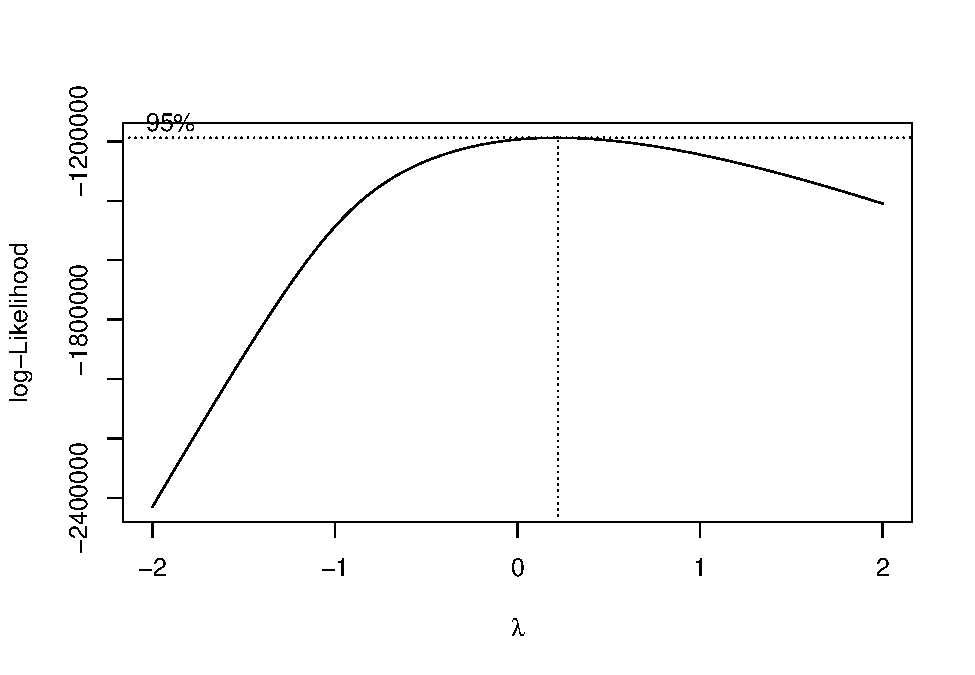
\includegraphics{Data_621_HW_1_files/figure-latex/unnamed-chunk-19-1.pdf}
\#\#\#\#\# Observations after removal of missing data * Although removal
of missing data resolves the distributions of many variables, the sample
size is reduced to under 10\% of the original dataset from 2276
observations to only 191 observations in the training dataset

\hypertarget{given-the-loss-of-data-with-the-removal-of-missing-data-the-most-appropriet-imputation-is-the-mean-and-we-should-proceed-with-that-method}{%
\subparagraph{Given the loss of data with the removal of missing data,
the most appropriet imputation is the mean and we should proceed with
that
method}\label{given-the-loss-of-data-with-the-removal-of-missing-data-the-most-appropriet-imputation-is-the-mean-and-we-should-proceed-with-that-method}}

\begin{Shaded}
\begin{Highlighting}[]
\CommentTok{\#print(skim(df\_train\_mn))}
\end{Highlighting}
\end{Shaded}

\begin{Shaded}
\begin{Highlighting}[]
\CommentTok{\#print(skim(df\_train\_md))}
\end{Highlighting}
\end{Shaded}

\begin{Shaded}
\begin{Highlighting}[]
\CommentTok{\#print(skim(df\_train\_0))}
\end{Highlighting}
\end{Shaded}

\hypertarget{correlation-with-response-variable}{%
\paragraph{Correlation with response
variable}\label{correlation-with-response-variable}}

\begin{Shaded}
\begin{Highlighting}[]
\NormalTok{df\_train\_mn }\SpecialCharTok{\%\textgreater{}\%} 
  \FunctionTok{gather}\NormalTok{(variable, value, TEAM\_BATTING\_H}\SpecialCharTok{:}\NormalTok{ TEAM\_FIELDING\_DP)}\SpecialCharTok{\%\textgreater{}\%} \CommentTok{\#pivot longer to plot all variables}
  \FunctionTok{ggplot}\NormalTok{(.,}\FunctionTok{aes}\NormalTok{(}\AttributeTok{x=}\NormalTok{value, }\AttributeTok{y=}\NormalTok{TARGET\_WINS)) }\SpecialCharTok{+} \CommentTok{\#plotting every variable}
  \FunctionTok{geom\_point}\NormalTok{(}\AttributeTok{color =} \StringTok{"grey"}\NormalTok{, }\AttributeTok{alpha =} \FloatTok{0.5}\NormalTok{) }\SpecialCharTok{+}
  \FunctionTok{geom\_smooth}\NormalTok{(}\AttributeTok{method =} \StringTok{"lm"}\NormalTok{, }\AttributeTok{se =} \ConstantTok{FALSE}\NormalTok{, }\AttributeTok{color =} \StringTok{"darkgreen"}\NormalTok{) }\SpecialCharTok{+}
  \FunctionTok{facet\_wrap}\NormalTok{(}\SpecialCharTok{\textasciitilde{}}\NormalTok{ variable, }\AttributeTok{scales =} \StringTok{"free"}\NormalTok{, }\AttributeTok{ncol =} \DecValTok{4}\NormalTok{) }\SpecialCharTok{+}
  \FunctionTok{theme\_classic}\NormalTok{()}
\end{Highlighting}
\end{Shaded}

\begin{verbatim}
## `geom_smooth()` using formula = 'y ~ x'
\end{verbatim}

\includegraphics{Data_621_HW_1_files/figure-latex/unnamed-chunk-23-1.pdf}
\#\#\#\#\# Observations about correlations with TARGET\_WINS * None of
the variable appear very strongly correlated with \textbf{TARGET\_WINS},
but some the \textbf{TEAM\_PITCHING} variable have modest correlation *
Team batting variables appear to have no correlation with
\textbf{TARGET\_WINS}, with the exception of \textbf{TEAM\_BATTING\_H}
which has a modest positive correlation with wins

\hypertarget{checking-for-multicollinearity}{%
\paragraph{Checking for
multicollinearity}\label{checking-for-multicollinearity}}

\begin{Shaded}
\begin{Highlighting}[]
\NormalTok{df\_train\_mn }\SpecialCharTok{\%\textgreater{}\%} 
 \FunctionTok{select}\NormalTok{(}\SpecialCharTok{{-}}\NormalTok{INDEX) }\SpecialCharTok{\%\textgreater{}\%} 
  \FunctionTok{cor}\NormalTok{(.,) }\SpecialCharTok{\%\textgreater{}\%} 
  \FunctionTok{corrplot}\NormalTok{(.,}\AttributeTok{method =} \StringTok{"ellipse"}\NormalTok{, }\AttributeTok{type =} \StringTok{"lower"}\NormalTok{, }\AttributeTok{diag =} \ConstantTok{FALSE}\NormalTok{)}
\end{Highlighting}
\end{Shaded}

\includegraphics{Data_621_HW_1_files/figure-latex/unnamed-chunk-24-1.pdf}
\#\#\#\#\# Observations about correlations with TARGET\_WINS * The
correlogram confirms that none of the variable are very strongly
correlated with \textbf{TARGET\_WINS}, with the exception of
\textbf{TEAM\_BATTING\_H} which has a modest positive correlation with
wins * Strong multicollinearity is seen between the following variable
which needs to be taken into consideration when constructing the models:
\textbf{TEAM\_FIELDING\_E}, \textbf{TEAM\_PITCHING\_HR},
\textbf{TEAM\_BATTING\_3B}, \textbf{TEAM\_BATTING\_HR} * It may also not
be advisable to include \textbf{TEAM\_BATTING\_HBP} in the model because
it has no correlation with wins or any other variable in the dataset

\hypertarget{models}{%
\subsection{\texorpdfstring{\textbf{Models}}{Models}}\label{models}}

\begin{Shaded}
\begin{Highlighting}[]
\NormalTok{model\_initial }\OtherTok{\textless{}{-}} \FunctionTok{lm}\NormalTok{(TARGET\_WINS }\SpecialCharTok{\textasciitilde{}}\NormalTok{ TEAM\_BATTING\_H}\SpecialCharTok{+}\NormalTok{TEAM\_BATTING\_2B }\SpecialCharTok{+}\NormalTok{TEAM\_BATTING\_3B}\SpecialCharTok{+}\NormalTok{TEAM\_BATTING\_HR}\SpecialCharTok{+}\NormalTok{TEAM\_BATTING\_BB}\SpecialCharTok{+}\NormalTok{TEAM\_BATTING\_SO}\SpecialCharTok{+}
\NormalTok{TEAM\_BASERUN\_SB}\SpecialCharTok{+}\NormalTok{ TEAM\_BASERUN\_CS }\SpecialCharTok{+}\NormalTok{ TEAM\_BATTING\_HBP }\SpecialCharTok{+}\NormalTok{TEAM\_PITCHING\_H}\SpecialCharTok{+}\NormalTok{ TEAM\_PITCHING\_HR}\SpecialCharTok{+}\NormalTok{TEAM\_PITCHING\_BB}\SpecialCharTok{+}\NormalTok{TEAM\_PITCHING\_SO}\SpecialCharTok{+}\NormalTok{TEAM\_FIELDING\_E}\SpecialCharTok{+}\NormalTok{ TEAM\_FIELDING\_DP, }\AttributeTok{data =}\NormalTok{ df\_train)}

\FunctionTok{summary}\NormalTok{(model\_initial)}
\end{Highlighting}
\end{Shaded}

\begin{verbatim}
## 
## Call:
## lm(formula = TARGET_WINS ~ TEAM_BATTING_H + TEAM_BATTING_2B + 
##     TEAM_BATTING_3B + TEAM_BATTING_HR + TEAM_BATTING_BB + TEAM_BATTING_SO + 
##     TEAM_BASERUN_SB + TEAM_BASERUN_CS + TEAM_BATTING_HBP + TEAM_PITCHING_H + 
##     TEAM_PITCHING_HR + TEAM_PITCHING_BB + TEAM_PITCHING_SO + 
##     TEAM_FIELDING_E + TEAM_FIELDING_DP, data = df_train)
## 
## Residuals:
##      Min       1Q   Median       3Q      Max 
## -19.8708  -5.6564  -0.0599   5.2545  22.9274 
## 
## Coefficients:
##                  Estimate Std. Error t value Pr(>|t|)    
## (Intercept)      60.28826   19.67842   3.064  0.00253 ** 
## TEAM_BATTING_H    1.91348    2.76139   0.693  0.48927    
## TEAM_BATTING_2B   0.02639    0.03029   0.871  0.38484    
## TEAM_BATTING_3B  -0.10118    0.07751  -1.305  0.19348    
## TEAM_BATTING_HR  -4.84371   10.50851  -0.461  0.64542    
## TEAM_BATTING_BB  -4.45969    3.63624  -1.226  0.22167    
## TEAM_BATTING_SO   0.34196    2.59876   0.132  0.89546    
## TEAM_BASERUN_SB   0.03304    0.02867   1.152  0.25071    
## TEAM_BASERUN_CS  -0.01104    0.07143  -0.155  0.87730    
## TEAM_BATTING_HBP  0.08247    0.04960   1.663  0.09815 .  
## TEAM_PITCHING_H  -1.89096    2.76095  -0.685  0.49432    
## TEAM_PITCHING_HR  4.93043   10.50664   0.469  0.63946    
## TEAM_PITCHING_BB  4.51089    3.63372   1.241  0.21612    
## TEAM_PITCHING_SO -0.37364    2.59705  -0.144  0.88577    
## TEAM_FIELDING_E  -0.17204    0.04140  -4.155 5.08e-05 ***
## TEAM_FIELDING_DP -0.10819    0.03654  -2.961  0.00349 ** 
## ---
## Signif. codes:  0 '***' 0.001 '**' 0.01 '*' 0.05 '.' 0.1 ' ' 1
## 
## Residual standard error: 8.467 on 175 degrees of freedom
##   (2085 observations deleted due to missingness)
## Multiple R-squared:  0.5501, Adjusted R-squared:  0.5116 
## F-statistic: 14.27 on 15 and 175 DF,  p-value: < 2.2e-16
\end{verbatim}

\hypertarget{reference}{%
\subsubsection{Reference}\label{reference}}

\begin{itemize}
\tightlist
\item
  ``Pythagorean Theorem of Baseball.'' Baseball Reference,
  \url{https://www.baseball-reference.com/bullpen/Pythagorean_Theorem_of_Baseball}.
  Accessed 11 September 2023.
\item
  No author listed. ``Pythagorean Expectation in Major League
  Baseball.'' Digital Commons @ Cal Poly,
  \url{https://digitalcommons.calpoly.edu/cgi/viewcontent.cgi?article=1067\&context=statsp}.
  Accessed 11 September 2023.
\end{itemize}

\end{document}
